%%%%%%%%%%%%%%%%%%%%%%%%%%%%%%%%%%%%%%%%%%%%%%%%%%%%%%%%%%%%%%%%%
\chapter{SIMULATION RESULTS}\label{ch:simulation_results}
%%%%%%%%%%%%%%%%%%%%%%%%%%%%%%%%%%%%%%%%%%%%%%%%%%%%%%%%%%%%%%%%%

For simulation results in this thesis, global simulation parameters are set as follows: packet size = 60 Bytes and simulation duration = 3600 seconds. First, single gateway and multiple gateway LoRaWAN network simulation results are presented to show correctness of the simulator, then, smart spreading factor scheme simulation results are presented.

\section{Single Gateway}

In Figure \ref{fig:sf}, PDR and transmit energy consumption plots of various spreading factor assignment schemes are shown. Randomly generated network topology radius is set to 3000 meters, number of gateways is set to 1 and packet generation rate is set to 0.01 pps. Increasing spreading factors increases air time. This increases the number of collisions thus decreases the PDR. High spreading factor schemes gives poor PDR results as the number of nodes increases. Since network topology radius is quite small, all spreading factors can reach to gateway.

\begin{figure}[h]
\centering
\subfigure[PDR]{
\label{fig:sf_pdr}
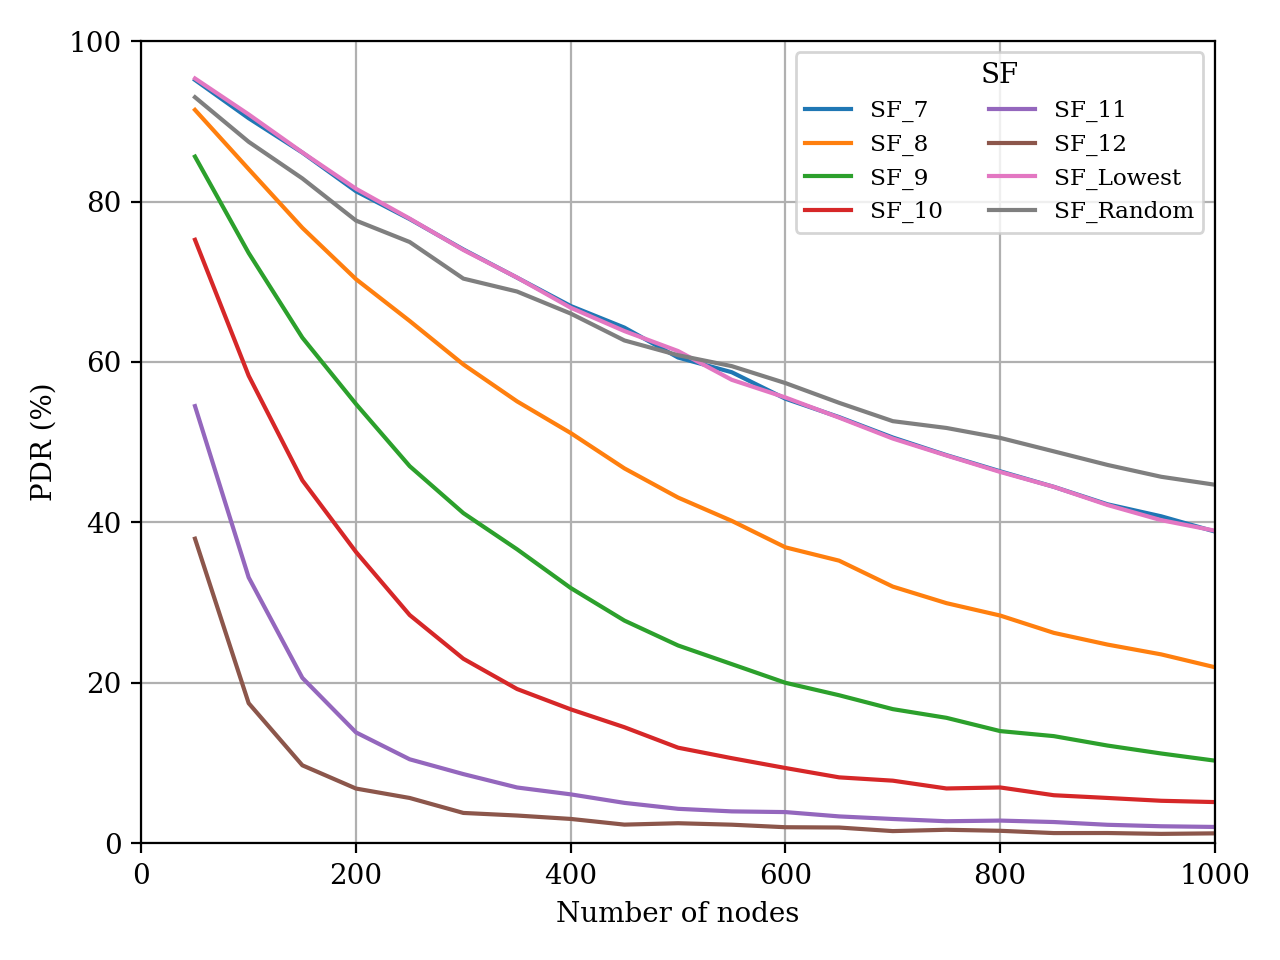
\includegraphics[width=.7\linewidth]{{fig/sf_pdr_r3000_g1_p0.01_s3600}.png}} \\
\subfigure[Transmit energy]{
\label{fig:sf_energy}
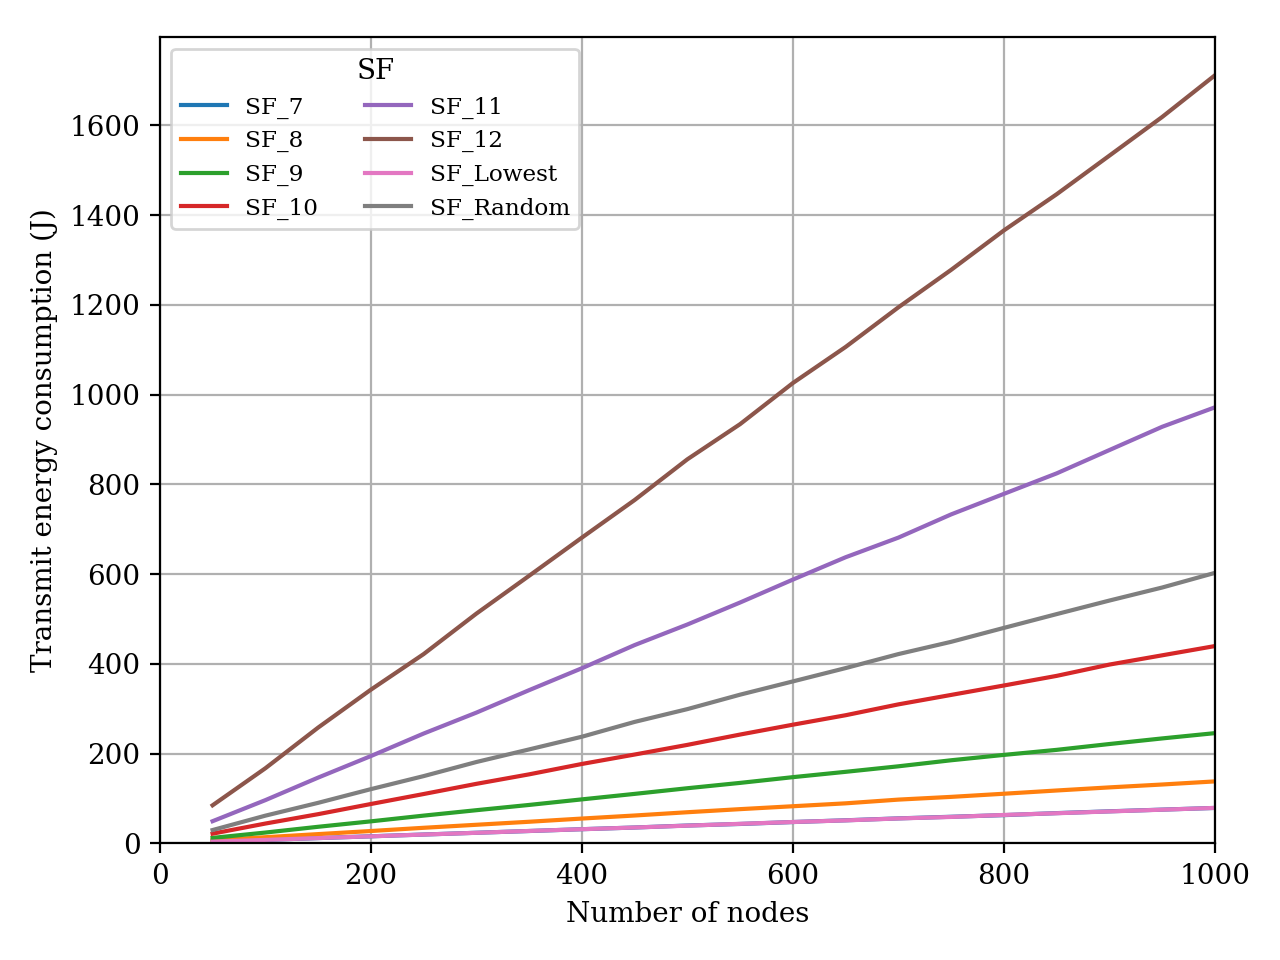
\includegraphics[width=.7\linewidth]{{fig/sf_energy_r3000_g1_p0.01_s3600}.png}}
\caption{Various spreading factors. (r = 3000 m, GW = 1, ${R_{b}}$ = 0.01 pps)}
\label{fig:sf}
\end{figure}

In Figure \ref{fig:r}, PDR and transmit energy consumption plots of various network radii are shown. Number of gateways is set to 1, lowest spreading factor assignment scheme is used and packet generation rate is set to 0.01 pps. Increasing network radius, increases the number of under sensitivity transmissions thus decreases the PDR of network.

\begin{figure}[h]
\centering
\subfigure[PDR]{
\label{fig:r_pdr}
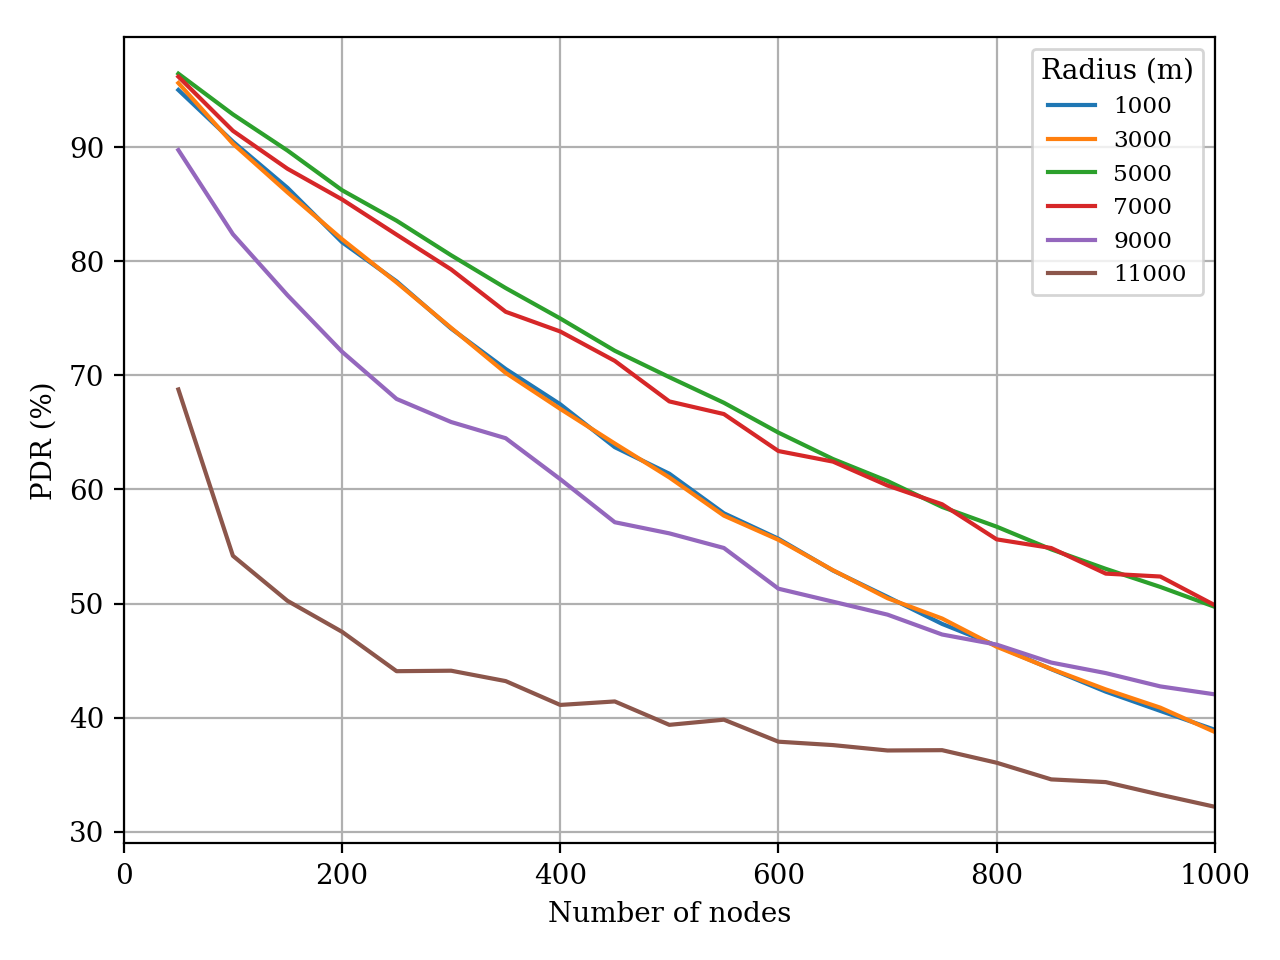
\includegraphics[width=.7\linewidth]{{fig/r_pdr_g1_p0.01_s3600}.png}} \\
\subfigure[Transmit energy]{
\label{fig:r_energy}
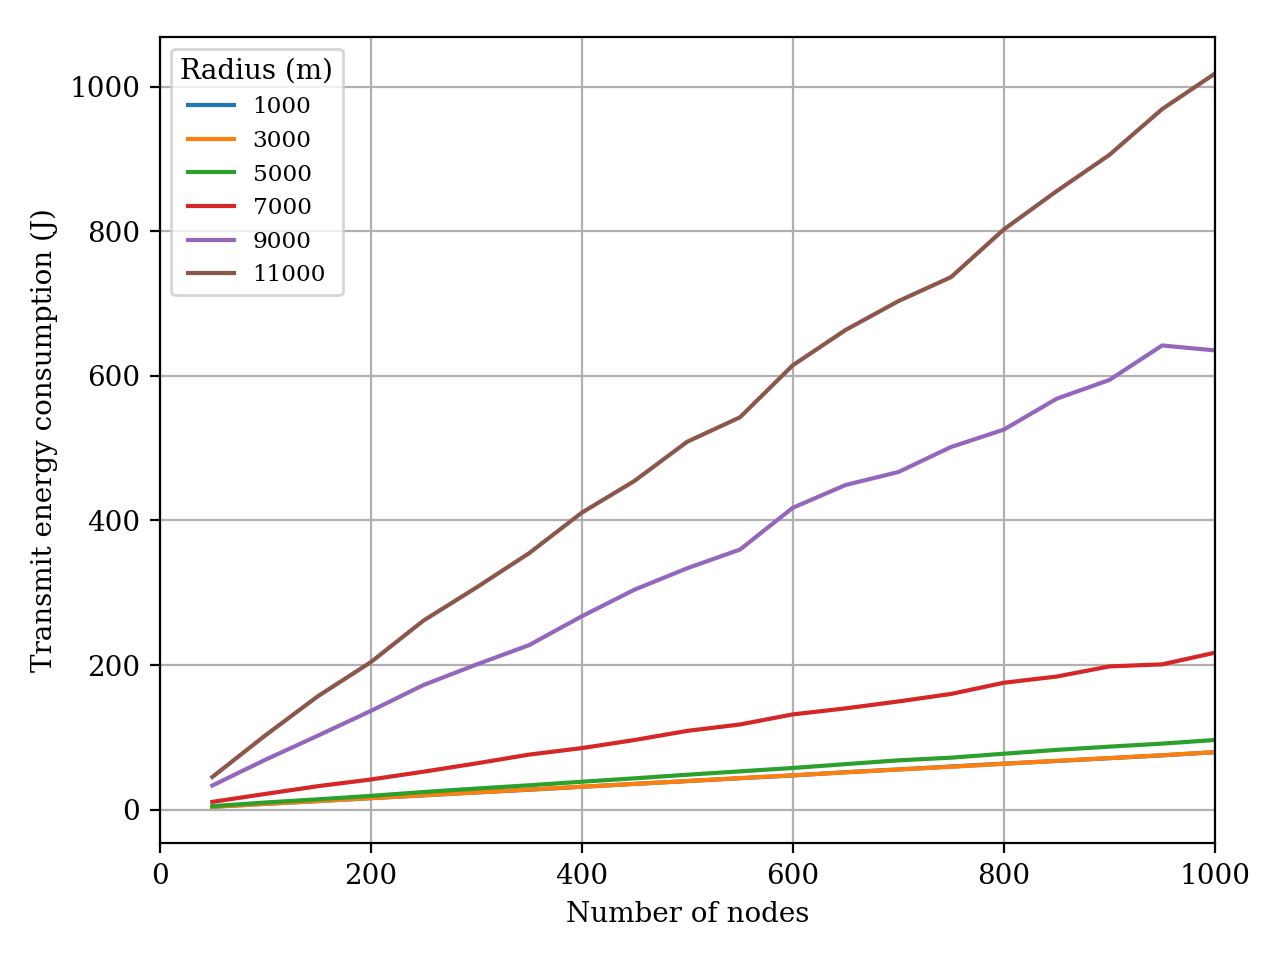
\includegraphics[width=.7\linewidth]{{fig/r_energy_g1_p0.01_s3600}.png}}
\caption{Various network radii. (GW = 1, SF = SF{\_}Lowest, ${R_{b}}$ = 0.01 pps)}
\label{fig:r}
\end{figure}

\par In Figure \ref{fig:pr}, PDR and transmit energy consumption plots of various packet generation rate are shown. Randomly generated topology radius is set to 3000 meters, number of gateways is set to 1 and lowest spreading factor assignment scheme is used. Increasing packet generation rate, increases the number of collisions thus decreases the PDR of network.

\begin{figure}[h]
\centering
\subfigure[PDR]{
\label{fig:pr_pdr}
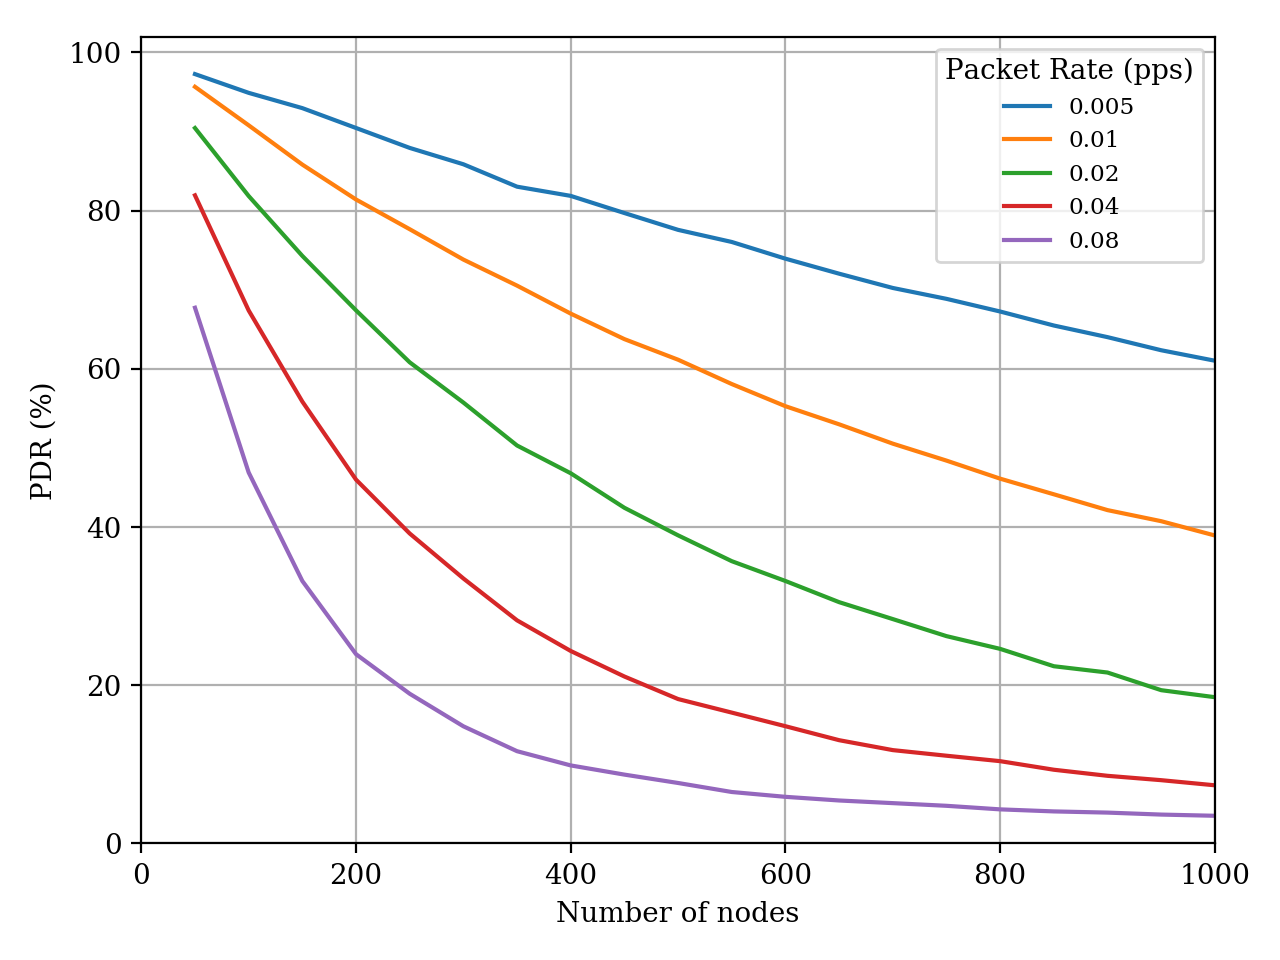
\includegraphics[width=.7\linewidth]{{fig/pr_pdr_r3000_g1_s3600}.png}} \\
\subfigure[Transmit energy]{
\label{fig:pr_energy}
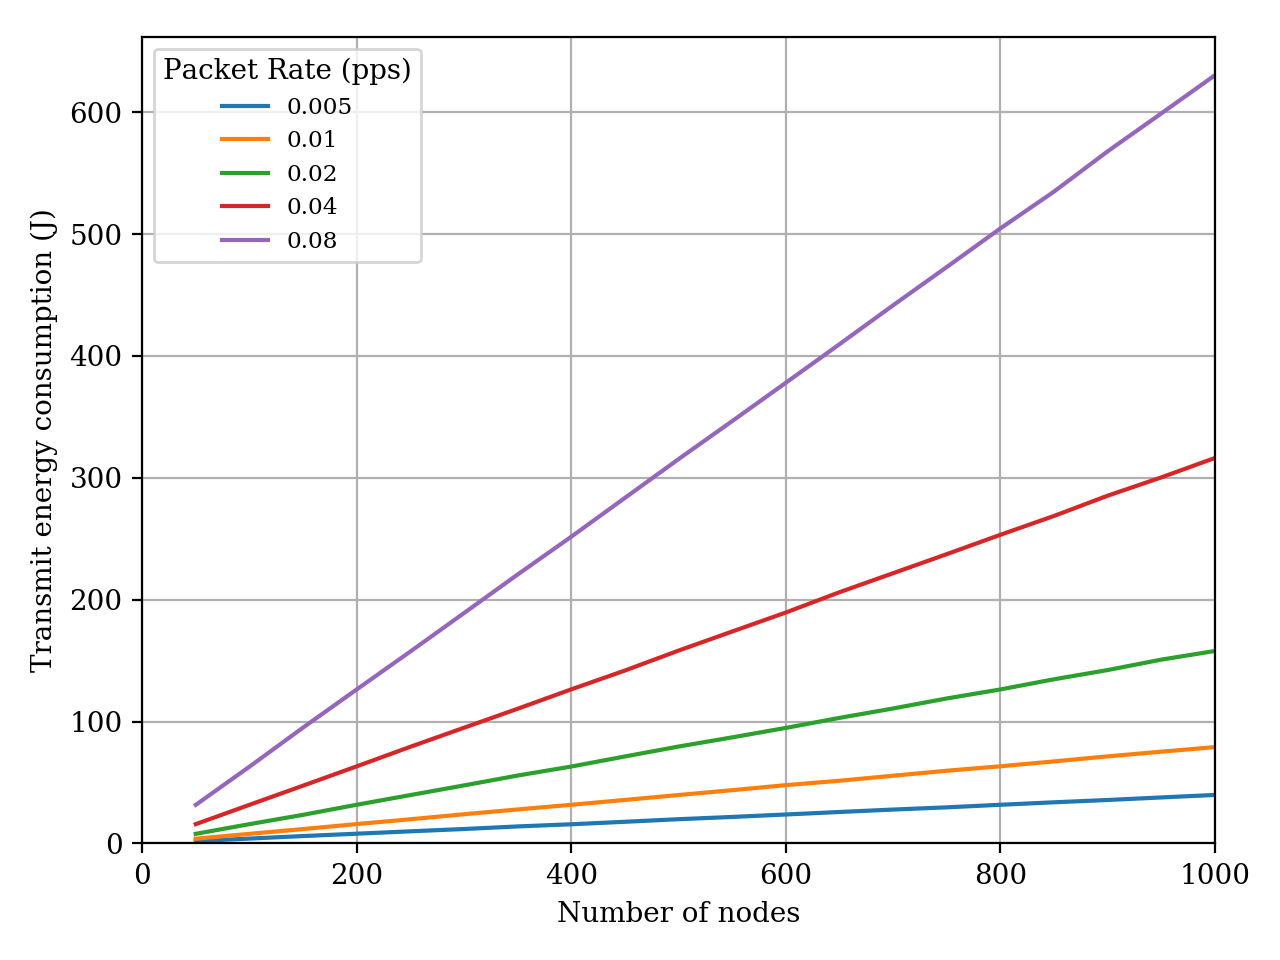
\includegraphics[width=.7\linewidth]{{fig/pr_energy_r3000_g1_s3600}.png}}
\caption{Various packet generation rates. (r = 5000 m, GW = 1, SF = SF{\_}Lowest)}
\label{fig:pr}
\end{figure}

\section{Multiple Gateway}

In Figure \ref{fig:gw}, PDR and transmit energy consumption plots for various number of gateways are shown. Randomly generated topology radius is set to 3000 meters, the lowest spreading factor assignment scheme is used and  packet generation rate is set to 0.01 pps. Increasing number of gateways, decreases the spreading factors of nodes and decreases air time. This decreases number of collisions, hence, increases the PDR of network when network radius is constant.

\begin{figure}[h]
\centering
\subfigure[PDR]{
\label{fig:gw_pdr}
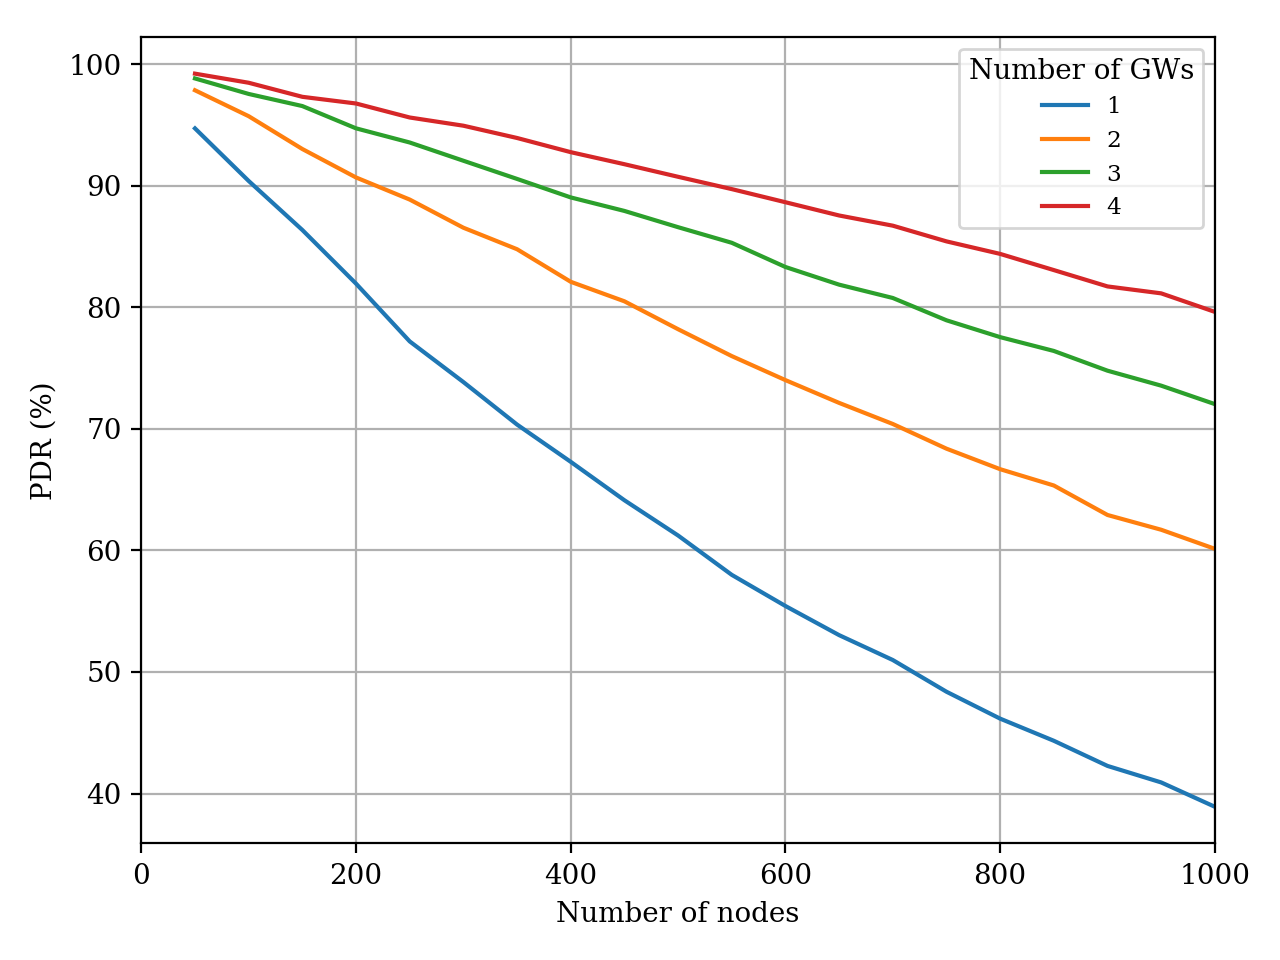
\includegraphics[width=.7\linewidth]{{fig/gw_pdr_r3000_p0.01_s3600}.png}} \\
\subfigure[Transmit energy]{
\label{fig:gw_energy}
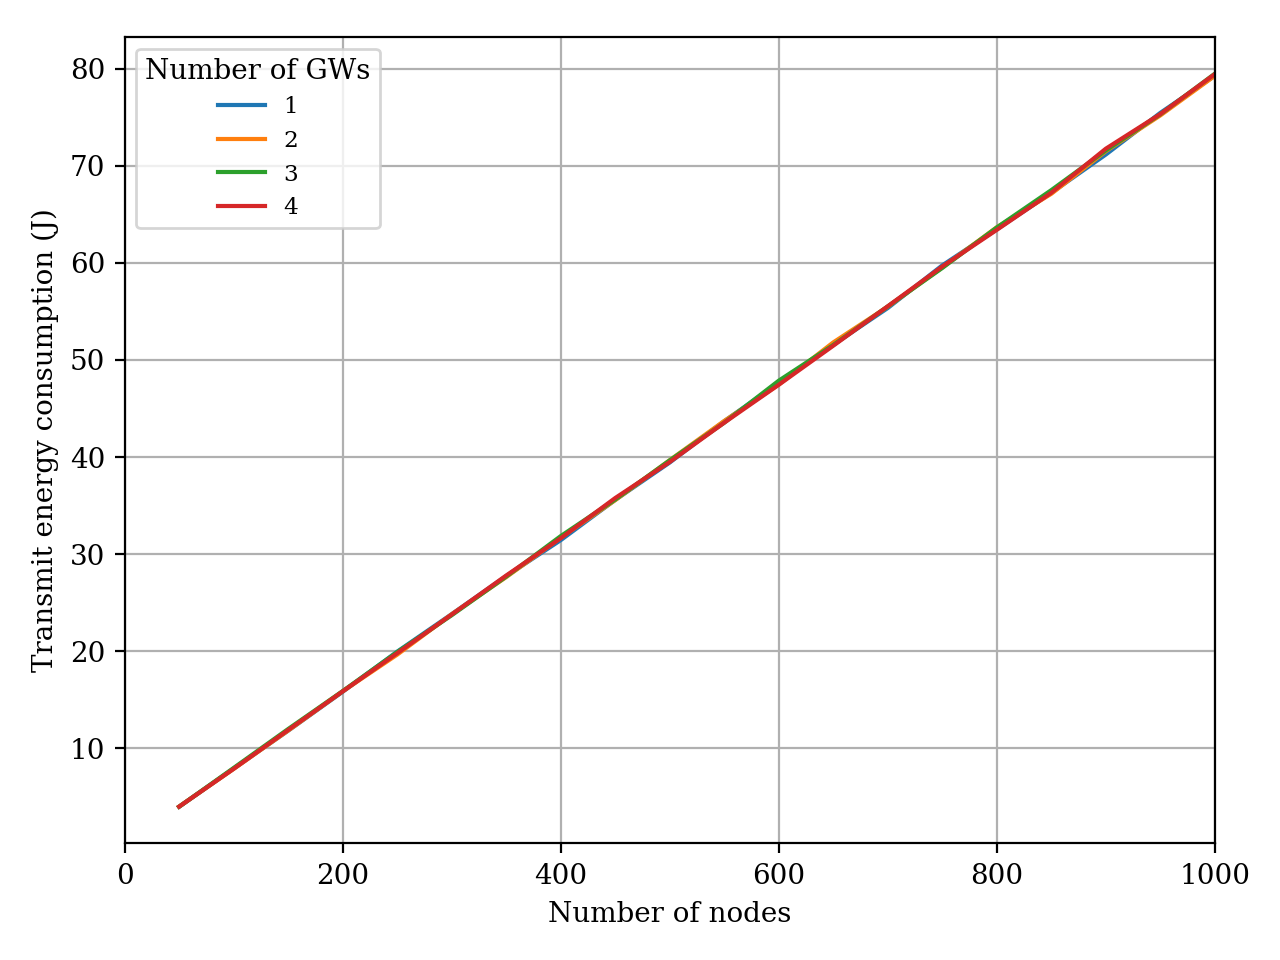
\includegraphics[width=.7\linewidth]{{fig/gw_energy_r3000_p0.01_s3600}.png}}
\caption{Various number of gateways. (r = 3000 m, SF = SF{\_}Lowest, ${R_{b}}$ = 0.01 pps)}
\label{fig:gw}
\end{figure}

\section{Smart Spreading Factor Schemes}

PDR and transmit energy plots of the lowest spreading factor, random spreading factor and the smart prediction schemes are shown in Figure \ref{fig:prediction}. Randomly generated network radius is set to 5000 meters, number of gateways is set to 3 and packet generation rate is set to 0.01 pps. Prediction model needs nodes' locations and three gateways are enough to locate position of nodes by triangulation. In Table \ref{table:prediction_pdr}, PDR values for various network radii are presented. Both smart SVM and smart DTC schemes give better PDR than lowest spreading factor schemes when number of nodes increases. Increasing number of nodes, increases number of interferences. Smart schemes improve network performance when LoRa interference is high. Moreover, smart schemes give better results when nodes are deployed closer to the gateway, since nodes have margin to increase their spreading factors when they are deployed closer to the gateway. If a node is far away from gateway, then smart schemes cannot increase the spreading factor to avoid interference since the assigned spreading factor is already high.

In Table \ref{table:prediction_accuracy}, prediction accuracy of smart SVM and smart DTC schemes are presented for various network radii and number of nodes. Prediction accuracy is not directly proportional to network PDR. Correct prediction of an interfered transmission may not increase the PDR but increases the prediction accuracy. Smart DTC gives better network PDR results than smart SVM, even overall smart SVM prediction accuracy is higher. The distribution of different labeled data points in the dataset is strongly related to simulation parameters. If simulation is run with small topology radius and high number of nodes, then number of interfered transmission labeled data points increases. On the other hand, using a large topology radius in the simulation causes the number of under sensitivity transmission labeled data points to increase. We choose moderately dense network parameters to bring it closer to real world deployments. With the simulation parameters utilized in this section, simulation usually produces imbalanced dataset. Number of under sensitivity transmission labeled data points are less than number of successful transmission labeled data points. Besides, number of interfered transmission labeled data points are even less then number of under sensitivity transmission labeled data points. In this case, smart DTC predicts interfered transmission labeled data points more accurately. Correct classification of interfered transmissions yields better network PDR results, thus smart DTC scheme gives better network PDR results.

\begin{figure}[h]
\centering
\subfigure[PDR]{
\label{fig:prediction_pdr}
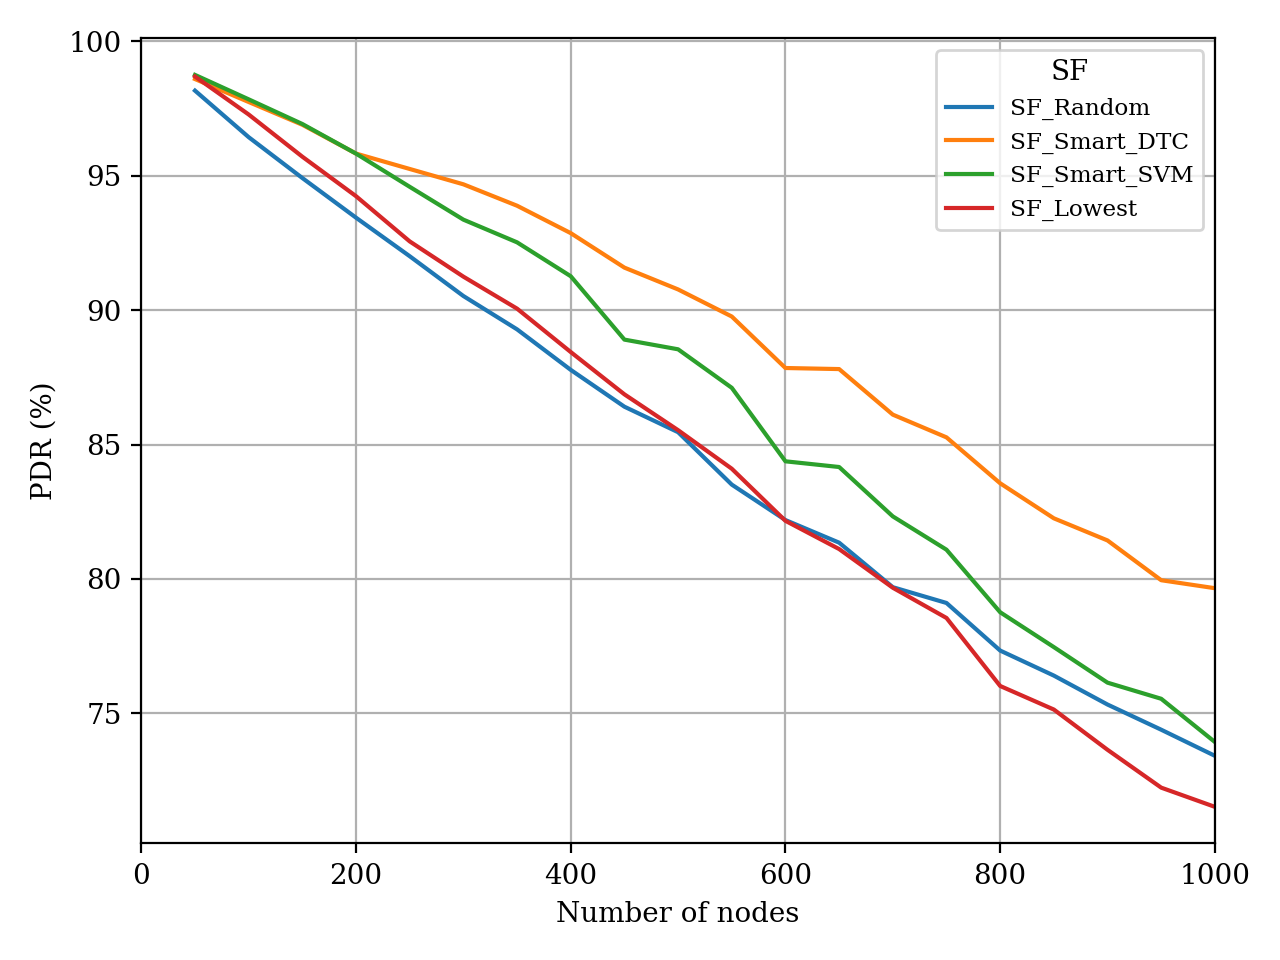
\includegraphics[width=.7\linewidth]{{fig/prediction_pdr_r5000_g3_p0.01_s3600}.png}} \\
\subfigure[Transmit energy]{
\label{fig:prediction_energy}
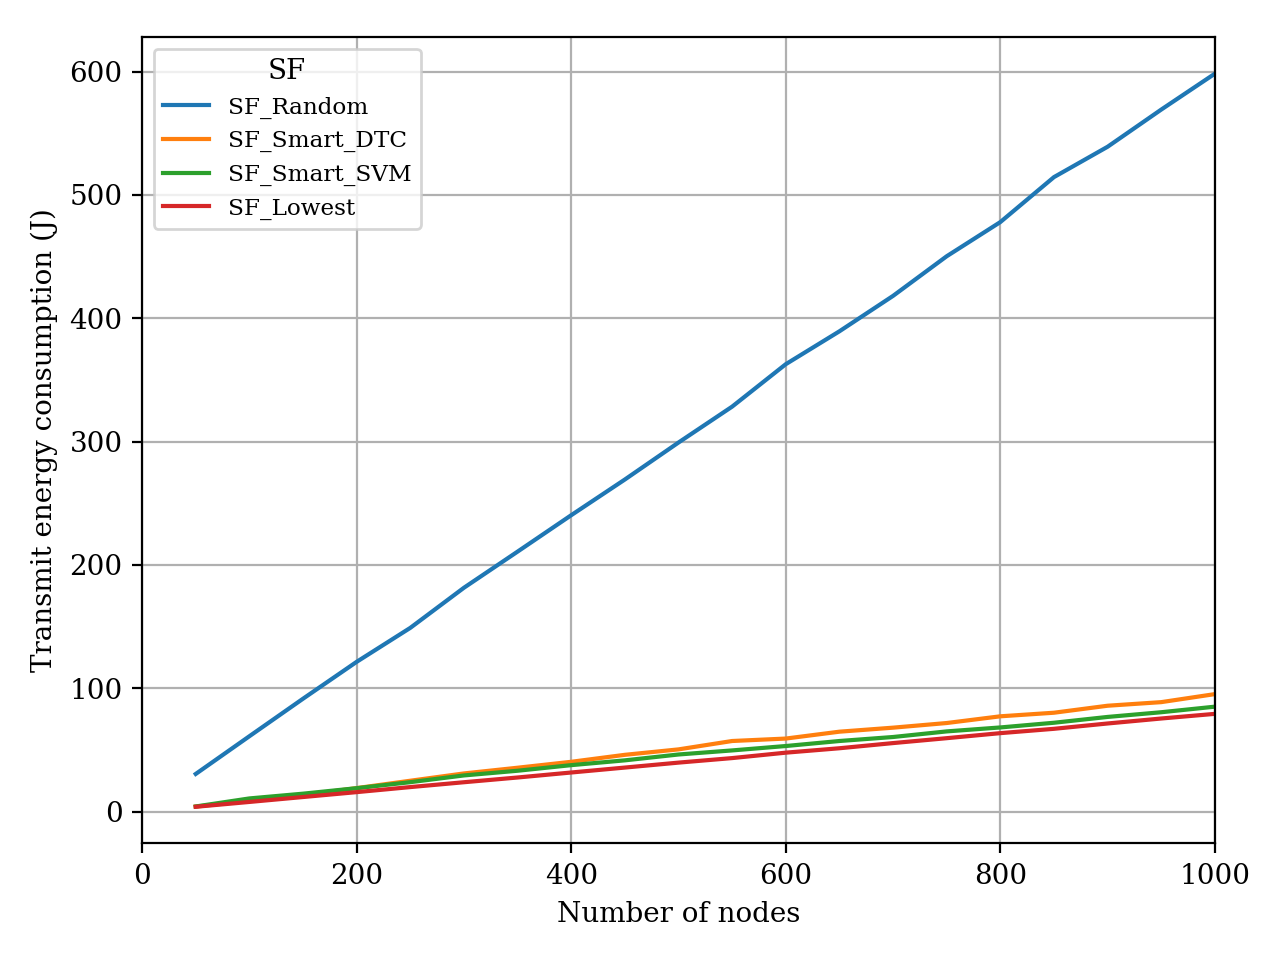
\includegraphics[width=.7\linewidth]{{fig/prediction_energy_r5000_g3_p0.01_s3600}.png}}
\caption{Lowest and smart spreading factor schemes. (r = 5000 m, GW = 3, ${R_{b}}$ = 0.01)}
\label{fig:prediction}
\end{figure}

\begin{table}[h]
\centering
\caption{PDR for lowest and smart spreading factor schemes. (GW = 3, ${R_{b}}$ = 0.01)}
\label{table:prediction_pdr}
\begin{tabular}{|c|c|c|c|c|c|}
\hline
\multicolumn{3}{|c|}{\multirow{2}{*}{}}                            & \multicolumn{3}{c|}{\textbf{Number of Nodes}} \\ \cline{4-6}
\multicolumn{3}{|c|}{}                                             & 100           & 500           & 1000          \\ \hline
\multirow{12}{*}{\textbf{r (m)}} & \multirow{3}{*}{3000}  & Lowest & 97.8          & 86.0          & 72.3          \\ \cline{3-6}
                                 &                        & SVM    & 98.0          & 88.2          & 75.2          \\ \cline{3-6}
                                 &                        & DTC    & 97.8          & 89.8          & 78.7          \\ \cline{2-6}

                                 & \multirow{3}{*}{5000}  & Lowest & 96.8          & 85.5          & 71.2          \\ \cline{3-6}
                                 &                        & SVM    & 98.0          & 87.8          & 74.8          \\ \cline{3-6}
                                 &                        & DTC    & 97.7          & 90.2          & 79.8          \\ \cline{2-6}

                                 & \multirow{3}{*}{7000}  & Lowest & 97.2          & 87.5          & 76.8          \\ \cline{3-6}
                                 &                        & SVM    & 98.2          & 88.8          & 78.6          \\ \cline{3-6}
                                 &                        & DTC    & 97.8          & 90.7          & 81.6          \\ \cline{2-6}

                                 & \multirow{3}{*}{10000} & Lowest & 98.2          & 90.3          & 81.5          \\ \cline{3-6}
                                 &                        & SVM    & 98.3          & 90.3          & 81.9          \\ \cline{3-6}
                                 &                        & DTC    & 98.3          & 90.6          & 81.9          \\ \hline
\end{tabular}
\end{table}

\begin{table}[h]
\centering
\caption{Prediction accuracy for SVM and DTC. (GW = 3, ${R_{b}}$ = 0.01))}
\label{table:prediction_accuracy}
\begin{tabular}{|c|c|c|c|c|c|}
\hline
\multicolumn{3}{|c|}{\multirow{2}{*}{}}                        & \multicolumn{3}{c|}{\textbf{Number of Nodes}} \\ \cline{4-6}
\multicolumn{3}{|c|}{}                                         & 100           & 500           & 1000          \\ \hline
\multirow{8}{*}{\textbf{r (m)}} & \multirow{2}{*}{3000}  & SVM & 82.4          & 70.4          & 71.7          \\ \cline{3-6}
                                &                        & DTC & 86.0          & 67.3          & 70.4          \\ \cline{2-6}

                                & \multirow{2}{*}{5000}  & SVM & 79.5          & 69.0          & 71.1          \\ \cline{3-6}
                                &                        & DTC & 84.5          & 67.3          & 69.5          \\ \cline{2-6}

                                & \multirow{2}{*}{7000}  & SVM & 79.5          & 70.6          & 71.2          \\ \cline{3-6}
                                &                        & DTC & 84.5          & 67.7          & 69.2          \\ \cline{2-6}

                                & \multirow{2}{*}{10000} & SVM & 79.2          & 74.4          & 76.1          \\ \cline{3-6}
                                &                        & DTC & 83.8          & 70.7          & 74.3          \\ \hline
\end{tabular}
\end{table}

% TODO add confusion matrices.

Readers are kindly invited to experiment the simulation tool with the parameters they like \cite{tugrul_yatagan_2019_2579366}.
